\documentclass[main.tex]{subfile}
%\documentclass[a4paper,8pt]{extarticle}
\begin{document}

\tiny
\subsection{Zero Order}
% subsection  (end)
$ a_0x = f(t) $ , $x(t) = \frac{1}{a_0} f(t)$ , $\frac{1}{a_0}$ static sensitivity

%\subsection{First Order}
%\label{sec:second_order}

$a_1\mathcal{D}^1x + a_0x = f(t)$

\begin{align}
	x(0) &= x_0
	, f(t) = 
	\begin{cases}
		A, & t \geq 0
		\\0, & < 0
	\end{cases}
	\\ & \iff x(t) = \frac{A}{a_0} + (x_0 - \frac{A}{a_0})e^{-t/\tau}
	\\f(t) &= Asin{\omega t}
	\\ & \iff x(t) = Ce^{-t/\tau} + \frac{A/a_0}{\sqrt{1 + (\omega\tau)^2}}
		\sin{\omega t - \tan^{-1}{\omega\tau}}
\end{align}

\begin{table}[H]
  \begin{center}
    \begin{tabular}{ll}
      \\ \toprule
			Time constant & $\tau = \frac{a_1}{a_0}$ 
			\\Rise Time & $e^{-t_1/\tau} = 0.1 \therefore t_1 \approx 2.303\tau$ 
			\\Phase shift angle & $\phi(\omega) = -tan^{-1}{\omega\tau}$
			\\Time delay & $\frac{\phi(\omega)}{\omega}$
      \\ \bottomrule
    \end{tabular}
  \end{center}
\end{table}

%\subsection{Second Order}
%\label{sec:second_order}

$m\mathcal{D}^2x + c\mathcal{D}^1x + kx = f(t)$

\begin{align}
	f(t) &= F_0\cos{\omega_1 t}
	\\ & \iff \left. x(t) = \frac{F_0/k}{\sqrt{(1-\alpha)^2 + \beta^2}} \cos{(\omega_1 t -
			\phi)} \right| \alpha = (\frac{\omega_1}{\omega_n})^2,\ \beta =
	2\xi\sqrt{\alpha},\ \xi = \frac{c}{c_c}
\end{align}

\begin{table}[H]
  \begin{center}
    \begin{tabular}{ll}
      \\ \toprule
			Phase angle & $\phi = \tan^{-1}{\frac{2\xi\sqrt{\alpha}}{1-\alpha}}$
			\\Natural Freq. & $\omega_n = \sqrt{k/m}$
			\\Critical Damping Coeff. & $c_c = 2\sqrt{mk}$
      \\ \bottomrule
    \end{tabular}
  \end{center}
\end{table}

% subsection second_order (end)

% subsection second_order (end)

%\subsection{Fourier Transform}
%\label{sec:fourier_transform}

\begin{align}
	y(x)  &= a_0 + \sum_{n=1}^{\infty} a_n\cos{nx} + b_n\sin{nx}
	\\a_0 &= \frac{1}{2L} \int_{-L}^{L} y(x)\ dx
	\\a_n &= \frac{1}{L} \int_{-L}^{L} y(x) \cos{n\pi x / L}\ dx
	\\b_n &= \frac{1}{L} \int_{-L}^{L} y(x) \sin{n\pi x / L}\ dx
\end{align}

% subsection fourier (end)

%\subsection{Other Functions}
%\label{sec:other_functions}

\begin{table}[H]
  \begin{center}
    \begin{tabular}{ll}
      \\ \toprule
			Saw tooth function & $F(t) = (\frac{2F_0}{T}t) $
      \\ \bottomrule
    \end{tabular}
  \end{center}
\end{table}

\begin{figure}
	\centering
	\begin{subfigure}{.5\linewidth}
		\centering
		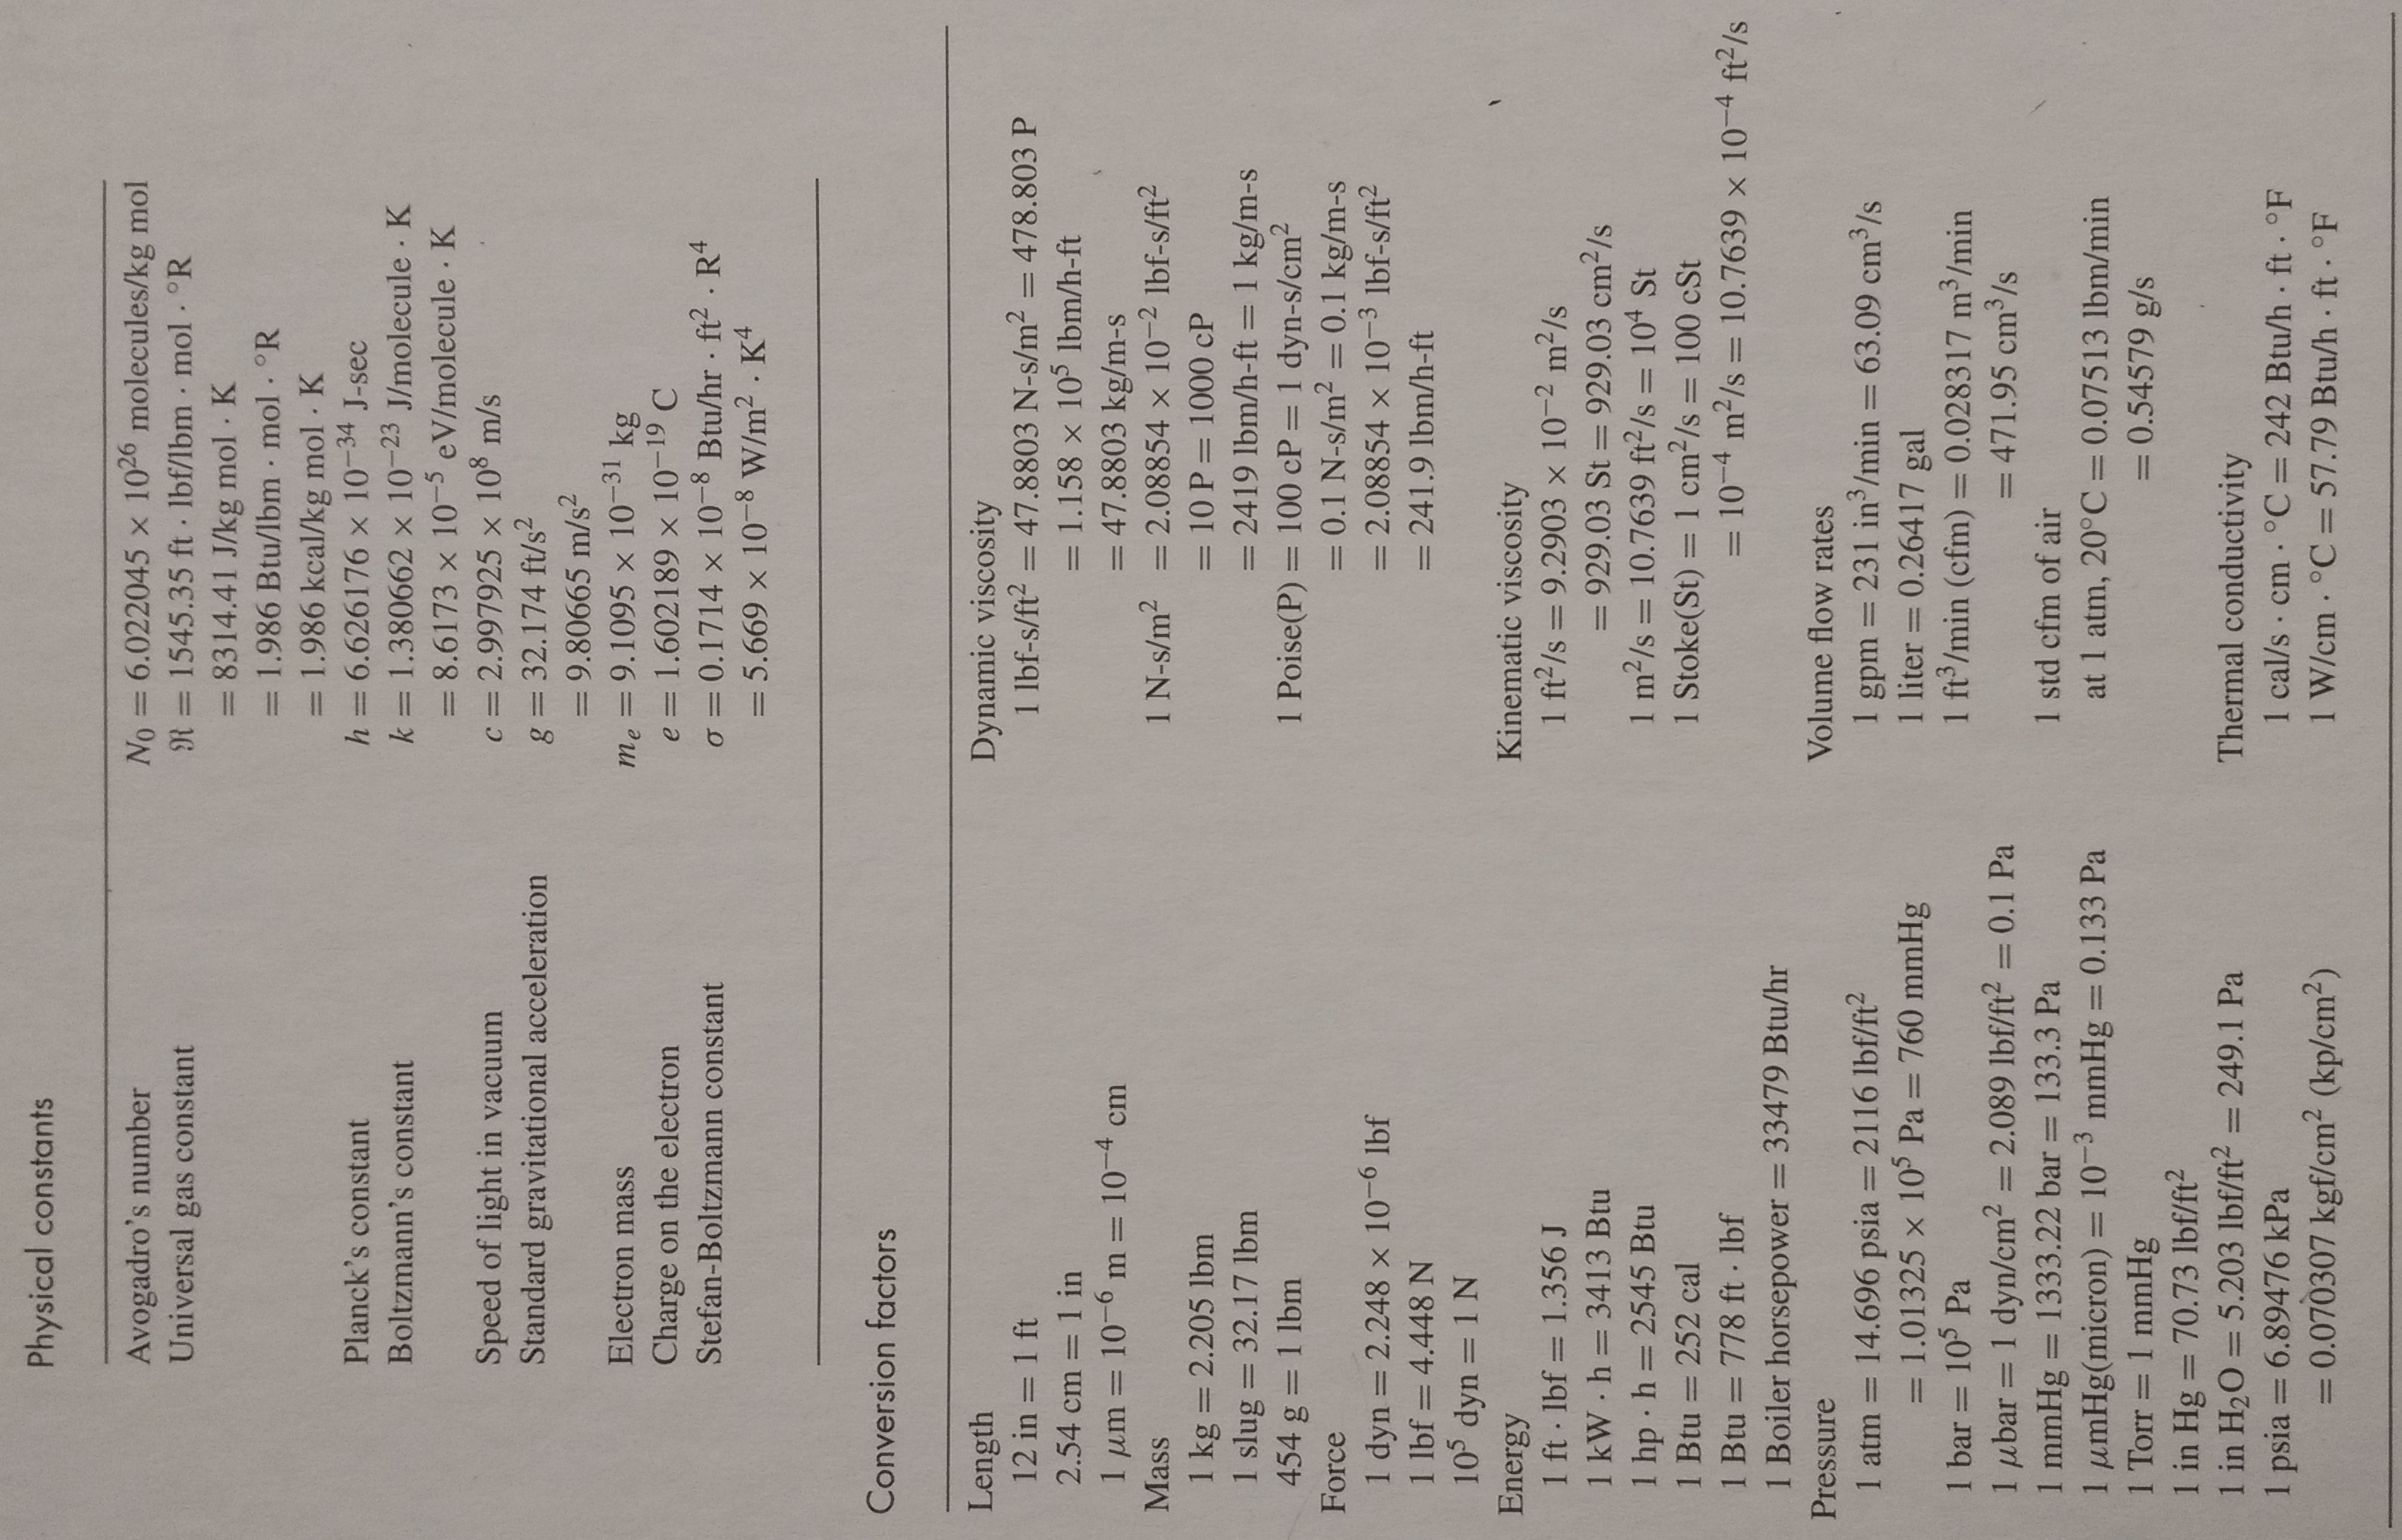
\includegraphics[angle=-90,width=.5\linewidth]{constants}
	\end{subfigure}%
	\begin{subfigure}{.5\linewidth}
		\centering
		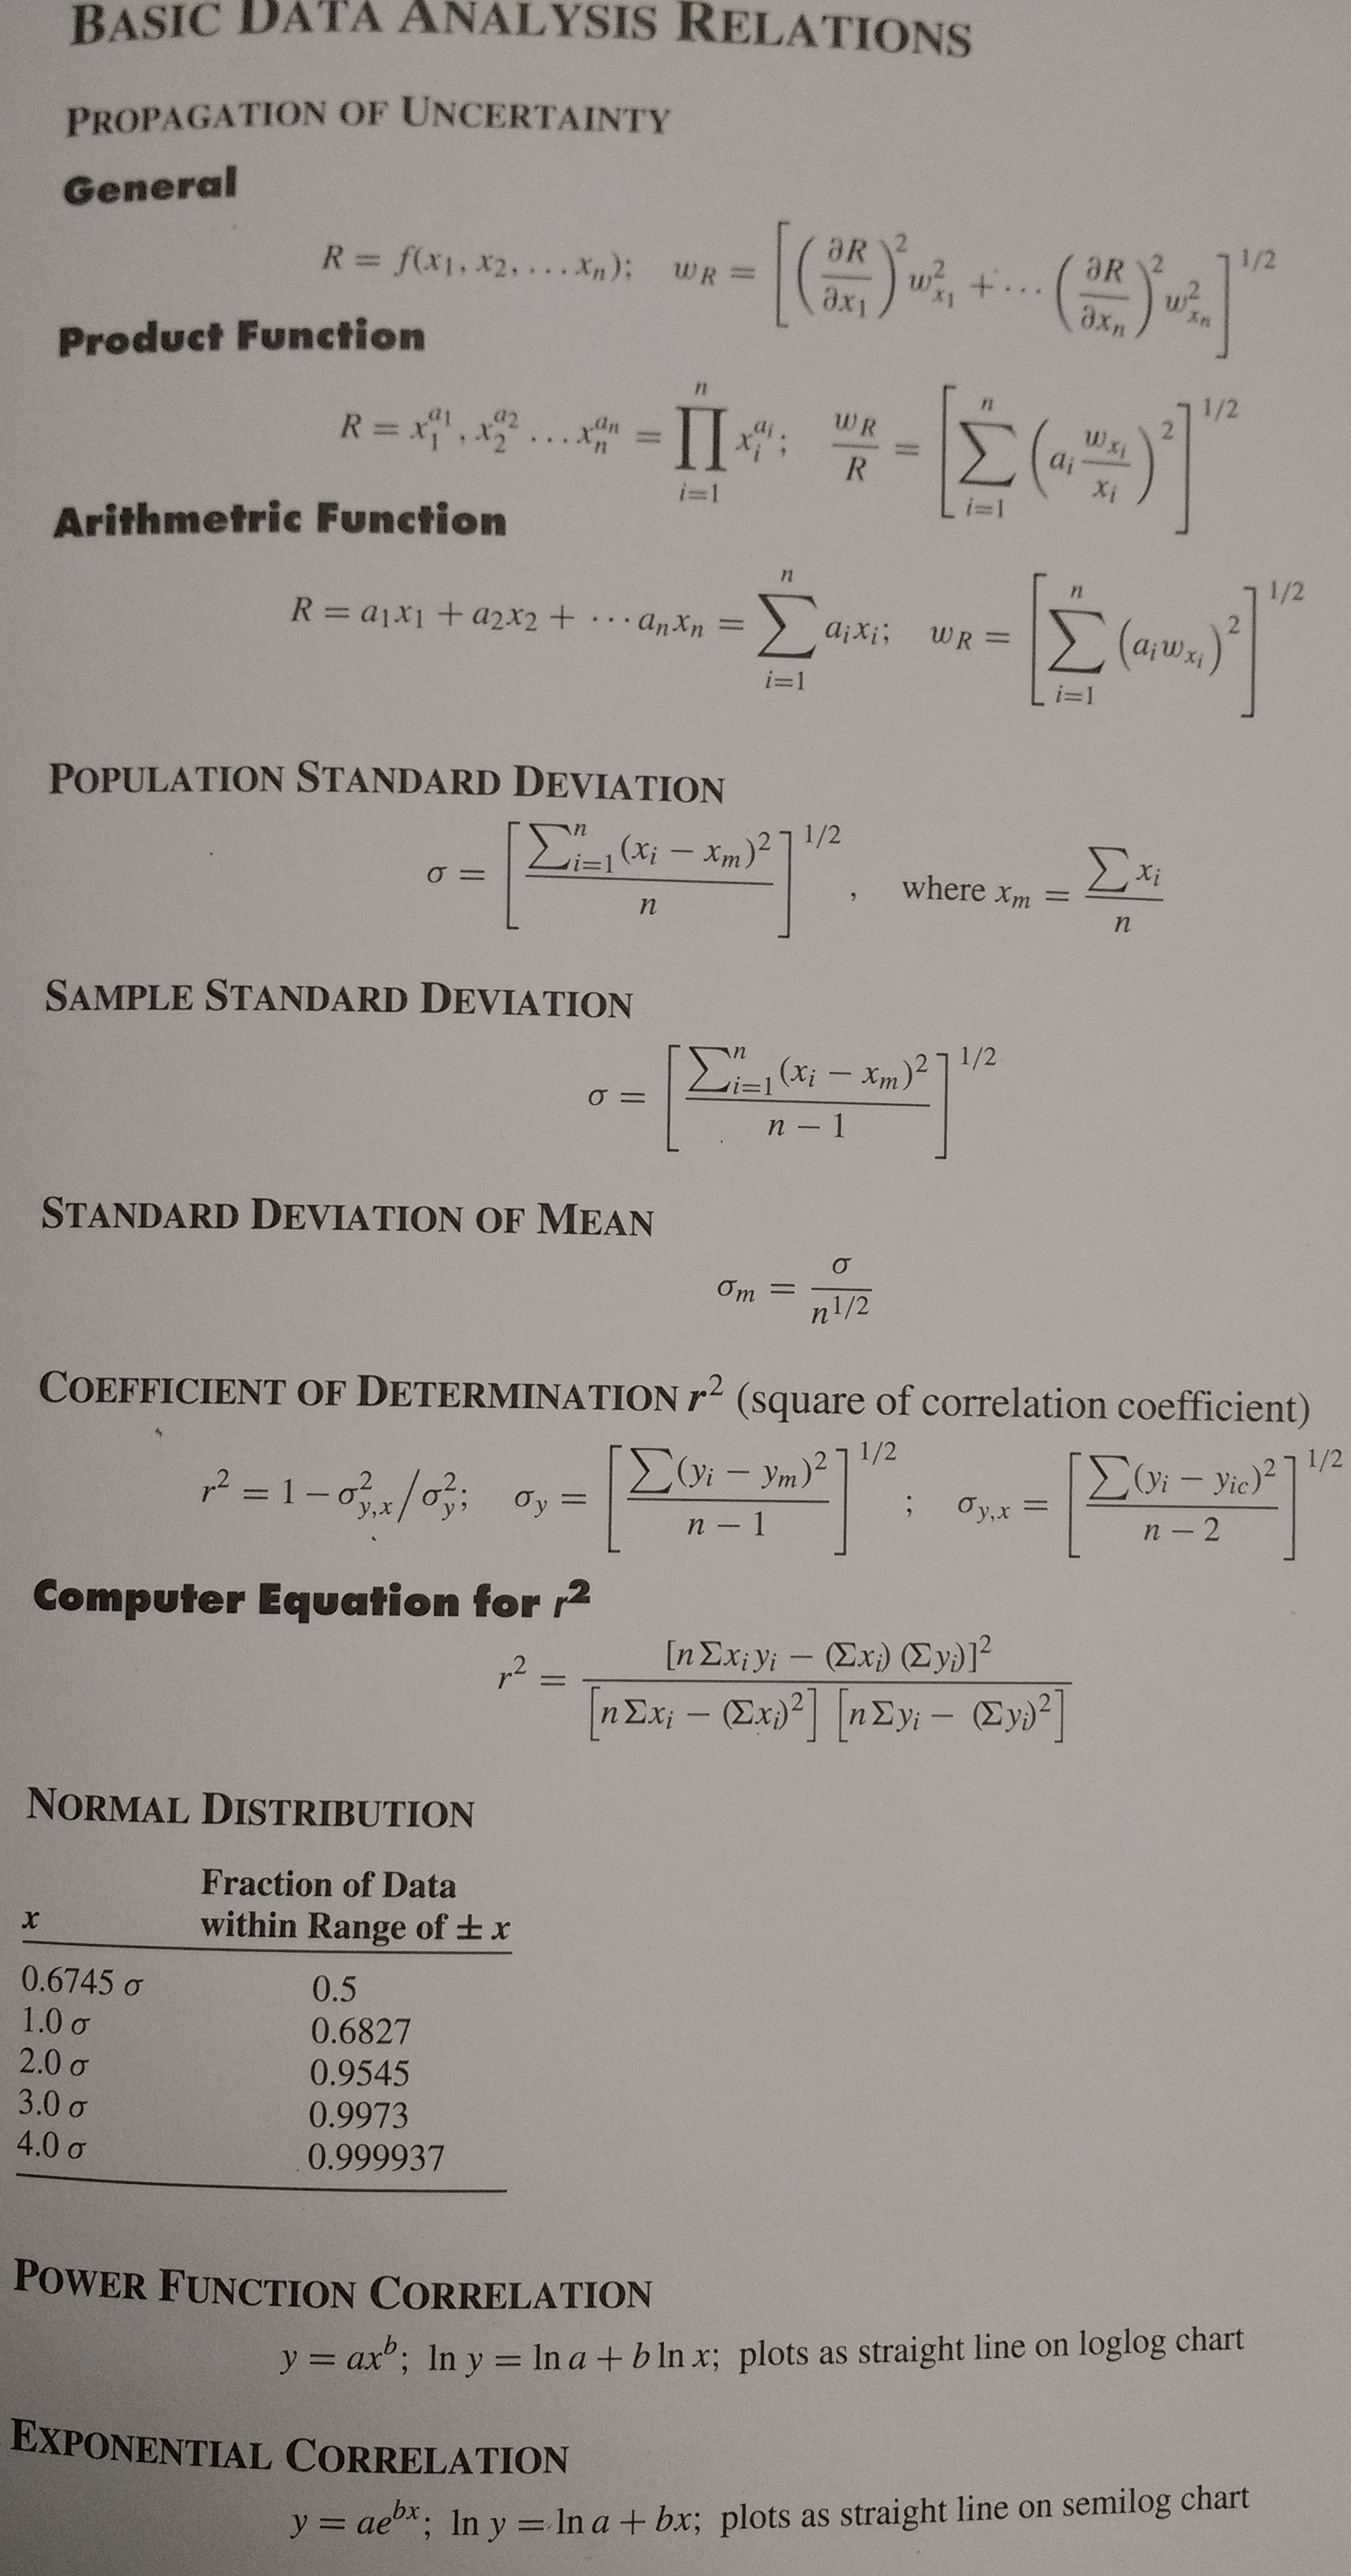
\includegraphics[width=.5\linewidth]{dataAnalysis}
	\end{subfigure}
\end{figure}


% subsection other_functions (end)

% subsection fourier_transform (end)

\end{document}
